% Common preamble for PIGMIE patent figures (A4).
% Drawing conventions:
%   - A4 portrait
%   - Sans-serif throughout (Helvetica)
%   - "Fig. N" sentence-case caption near top
%   - Page "N/total" at top centre
%   - Reference numerals outside boxes via leader lines
%   - ALL CAPS labels in component boxes
%   - Reactor uses north-east-lines hatched fill
%   - Scene uses double-line border
%   - Module enclosures use dashed line with internal numeral

\documentclass[a4paper,10pt]{article}
\usepackage[top=2.5cm,bottom=1.0cm,left=2.5cm,right=1.5cm]{geometry}
\usepackage[T1]{fontenc}
\usepackage{helvet}
\renewcommand{\familydefault}{\sfdefault}
\usepackage{amsmath,amssymb,bm}
\usepackage{tikz}
\usetikzlibrary{shapes,shapes.geometric,shapes.misc,arrows.meta,positioning,fit,calc,backgrounds,decorations.pathreplacing,decorations.markings,patterns}
\pagestyle{empty}
\setlength{\parindent}{0pt}

\tikzset{
  % Component box: ALL CAPS label inside, no numeral inside
  cbox/.style={draw, rectangle, minimum height=1.0cm, minimum width=2.4cm,
               align=center, line width=0.5pt, font=\small},
  cbox-tall/.style={cbox, minimum height=1.6cm},
  cbox-wide/.style={cbox, minimum width=3.0cm},
  cbox-narrow/.style={cbox, minimum width=1.8cm, font=\footnotesize},
  % Reactor / physical medium: hatched fill
  reactor/.style={cbox, pattern=north east lines, pattern color=black!70},
  % Scene: double-line border
  scenebox/.style={cbox, double, double distance=1.2pt, line width=0.4pt},
  % Module / sub-module enclosure
  enclosure/.style={draw, rectangle, dashed, line width=0.4pt, inner sep=10pt, rounded corners=2pt},
  enclosure-solid/.style={draw, rectangle, line width=0.5pt, inner sep=10pt, rounded corners=2pt},
  % Arrows
  flowarr/.style={-Latex, line width=0.5pt, font=\scriptsize},
  flowbi/.style={Latex-Latex, line width=0.5pt, font=\scriptsize},
  flowarr-fb/.style={-Latex, line width=0.5pt, dashed, font=\scriptsize},
  % Reference numeral leader-line endpoint and label
  refnum/.style={font=\footnotesize, inner sep=1pt},
  leader/.style={line width=0.4pt, -Latex},
  % Caption banner
  figcap/.style={font=\bfseries\large}
}

% Helper: figure header (page number + Fig. N caption)
\newcommand{\figheader}[3]{%
  % #1 = page number (e.g. "1"), #2 = total pages, #3 = figure label (e.g. "1" or "4A")
  \noindent\hfill\small #1/#2\hfill\null\par
  \vspace{0.2cm}
  \begin{center}\bfseries Fig.\ #3\end{center}
  \vspace{0.2cm}
}


\begin{document}

\figheader{4}{7}{4}

\begin{center}
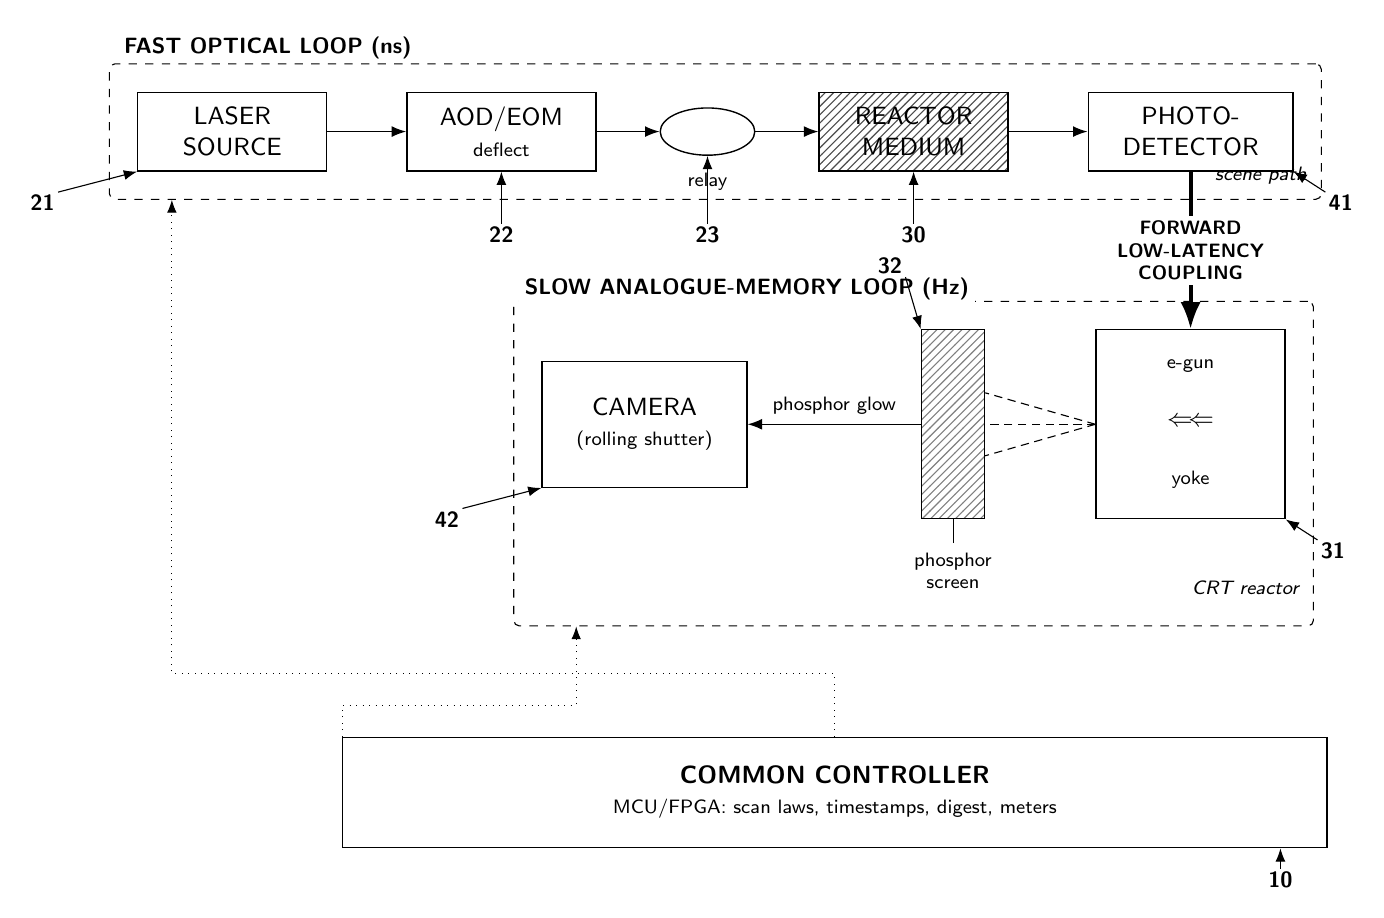
\begin{tikzpicture}[node distance=8mm]

% ============== TOP: FAST OPTICAL LOOP ==============
\node[cbox, minimum width=2.4cm] (laser) {LASER\\SOURCE};
\node[cbox, right=10mm of laser, minimum width=2.4cm] (aod) {AOD/EOM\\\scriptsize deflect};
\node[draw, ellipse, minimum width=1.2cm, minimum height=6mm, line width=0.5pt, right=8mm of aod] (relay) {};
\node[font=\scriptsize, below=1mm of relay] {relay};
\node[reactor, right=8mm of relay, minimum width=2.4cm] (react) {REACTOR\\MEDIUM};
\node[cbox, right=10mm of react, minimum width=2.6cm] (pd) {PHOTO-\\DETECTOR};

\draw[flowarr] (laser.east) -- (aod.west);
\draw[flowarr] (aod.east) -- (relay.west);
\draw[flowarr] (relay.east) -- (react.west);
\draw[flowarr] (react.east) -- (pd.west);

\begin{scope}[on background layer]
  \node[enclosure, fit=(laser)(aod)(relay)(react)(pd), inner sep=10pt] (fastloop) {};
\end{scope}
\node[font=\footnotesize\bfseries, anchor=south west] at ($(fastloop.north west)+(2pt,-2pt)$)
  {FAST OPTICAL LOOP (ns)};
\node[font=\scriptsize\itshape, anchor=south east] at ($(fastloop.south east)+(-2pt,2pt)$) {scene path};

% ============== BOTTOM: SLOW ANALOGUE-MEMORY LOOP (camera left, e-gun right under PD) ==============
% E-gun anchored directly below PD so the cascade forward coupling is a clean vertical line.
\node[cbox, below=20mm of pd, minimum width=2.4cm, minimum height=2.4cm, align=center] (egun)
  {\scriptsize e-gun\\[10pt]\textsf{$\Leftarrow\!\Leftarrow$}\\[10pt]\scriptsize yoke};
\node[draw, line width=0.5pt, pattern=north east lines, pattern color=black!50,
      left=14mm of egun, minimum width=8mm, minimum height=2.4cm] (phos) {};
% Phosphor screen label below the box (no longer a side label, since both sides have flow)
\node[font=\scriptsize, align=center, below=3mm of phos] (phoslabel) {phosphor\\screen};
\draw[line width=0.3pt] (phoslabel.north) -- (phos.south);
% Electron beam: e-gun (right) -> phosphor (left)
\draw[line width=0.4pt, densely dashed] (egun.west) -- ([yshift=4mm]phos.east);
\draw[line width=0.4pt, densely dashed] (egun.west) -- (phos.east);
\draw[line width=0.4pt, densely dashed] (egun.west) -- ([yshift=-4mm]phos.east);

\node[cbox-tall, left=22mm of phos, minimum width=2.6cm] (cam)
  {CAMERA\\\scriptsize (rolling shutter)};
% Phosphor glow: phosphor (right side of cam) -> camera (right-to-left visual flow)
\draw[flowarr] (phos.west) -- node[above, font=\scriptsize] {phosphor glow} (cam.east);

\begin{scope}[on background layer]
  \node[enclosure, fit=(egun)(phos)(cam)(phoslabel), inner sep=10pt] (slowloop) {};
\end{scope}
\node[font=\footnotesize\bfseries, anchor=south west, fill=white, inner sep=2pt] at ($(slowloop.north west)+(2pt,-2pt)$)
  {SLOW ANALOGUE-MEMORY LOOP (Hz)};
\node[font=\scriptsize\itshape, anchor=south east] at ($(slowloop.south east)+(-2pt,8pt)$) {CRT reactor};

% ============== CASCADE FORWARD COUPLING (embodiment b) ==============
% Heavy stroke arrow from PD straight DOWN into e-gun. Load-bearing forward
% path of the cascade embodiment: direct (optical via gain-pumped media, or
% electrical), low latency. With e-gun anchored below PD, the path is a
% clean vertical with no horizontal traversal.
\draw[-Latex, line width=1.5pt] (pd.south) -- (egun.north);
\node[font=\scriptsize\bfseries, align=center, fill=white, inner sep=2pt]
  at ($(pd.south)!0.5!(egun.north)$)
  {FORWARD\\LOW-LATENCY\\COUPLING};

% ============== COMMON CONTROLLER ==============
\node[cbox-wide, below=14mm of slowloop.south, xshift=-10mm,
      minimum width=12.5cm, minimum height=1.4cm] (ctrl)
  {\textbf{COMMON CONTROLLER}\\\scriptsize MCU/FPGA: scan laws, timestamps, digest, meters};

% Controller fan-out: dotted lines into the SOUTH corners of each loop
% Both routed to LEFT side of figure to avoid cascade column on the right
\draw[line width=0.35pt, dotted, -Latex] (ctrl.north west) -- ++(0,4mm) -| ($(slowloop.south west)+(8mm,0)$);
\draw[line width=0.35pt, dotted, -Latex] (ctrl.north) -- ++(0,8mm) -| ($(fastloop.south west)+(8mm,0)$);

% Reference numerals (positioned BELOW boxes / outside enclosures to avoid header collisions)
\node[refnum] at ($(laser.south west)+(-12mm,-4mm)$) (n21) {\textbf{21}};
\draw[leader] (n21.north east) -- (laser.south west);
\node[refnum] at ($(aod.south)+(0,-8mm)$) (n22) {\textbf{22}};
\draw[leader] (n22.north) -- (aod.south);
\node[refnum] at ($(relay.south)+(0,-10mm)$) (n23) {\textbf{23}};
\draw[leader] (n23.north) -- (relay.south);
\node[refnum] at ($(react.south)+(0,-8mm)$) (n30) {\textbf{30}};
\draw[leader] (n30.north) -- (react.south);
\node[refnum] at ($(pd.south east)+(6mm,-4mm)$) (n41) {\textbf{41}};
\draw[leader] (n41.north west) -- (pd.south east);

% Slow loop numerals for mirrored layout (cam left, phos middle, egun right)
\node[refnum] at ($(cam.south west)+(-12mm,-4mm)$) (n42) {\textbf{42}};
\draw[leader] (n42.north east) -- (cam.south west);
\node[refnum] at ($(phos.north)+(-8mm,8mm)$) (n32) {\textbf{32}};
\draw[leader] (n32.south east) -- (phos.north west);
\node[refnum] at ($(egun.south east)+(6mm,-4mm)$) (n31) {\textbf{31}};
\draw[leader] (n31.north west) -- (egun.south east);

\node[refnum] at ($(ctrl.south east)+(-6mm,-4mm)$) (n10) {\textbf{10}};
\draw[leader] (n10.north) -- ($(ctrl.south east)+(-6mm,0)$);

\end{tikzpicture}
\end{center}

\end{document}
